\documentclass[10pt,a4paper]{article}
\usepackage[bindingoffset=0.2in,%
            left=2.5cm,right=2cm,top=2.7cm,bottom=1in,%
            footskip=.25in]{geometry}
\usepackage[utf8]{inputenc}
\usepackage[ngerman]{babel}
\usepackage{amsmath, amsfonts, amssymb}
\usepackage{scrpage2}
\usepackage{color}
\usepackage{titlesec}
\pagestyle{scrheadings}
\usepackage{ulem, contour}
\usepackage{multicol}
\usepackage{hyperref}
\usepackage{listings}
\usepackage{pdfpages}
\usepackage{tabularx}
\usepackage{subcaption}
\usepackage{float}
\usepackage{scrextend}
\usepackage{enumerate}
\usepackage[bottom, splitrule]{footmisc}
\usepackage{multirow, enumitem}
\usepackage{csquotes}

\usepackage[style=authoryear, backend=biber]{biblatex}
\addbibresource{bibliography.bib}

\DeclareFixedFont{\ttb}{T1}{txtt}{bx}{n}{12} % for bold
\DeclareFixedFont{\ttm}{T1}{txtt}{m}{n}{12}  % for normal

\renewcommand{\ULdepth}{1.8pt}
\contourlength{0.8pt}

\newcommand{\cul}[1]{%
  \uline{\phantom{#1}}%
  \llap{\contour{white}{#1}}%
}

\graphicspath{
    {Images/}
}

\newrobustcmd*{\parentexttrack}[1]{%
  \begingroup
  \blx@blxinit
  \blx@setsfcodes
  \blx@bibopenparen#1\blx@bibcloseparen
  \endgroup}

\AtEveryCite{%
  \let\parentext=\parentexttrack%
  \let\bibopenparen=\bibopenbracket%
  \let\bibcloseparen=\bibclosebracket}

\definecolor{gray}{rgb}{0.33, 0.33, 0.33}
\definecolor{greengreen}{rgb}{0.0, 0.56, 0.0}
\definecolor{fgreen}{rgb}{0.13, 0.55, 0.13}
\definecolor{grellow}{rgb}{0.68, 1.0, 0.18}
\definecolor{orange}{rgb}{1.0, 0.49, 0.0}
\definecolor{deepblue}{rgb}{0,0,0.5}
\definecolor{deepred}{rgb}{0.6,0,0}
\definecolor{deepgreen}{rgb}{0,0.5,0}

\usepackage{pifont}

\newcommand{\cmark}{\ding{51}}%
\newcommand{\xmark}{\ding{55}}%
\newcommand{\wontfix}{\rlap{$\square$}{\large\hspace{1pt}\xmark}}

\makeatletter
\newcommand*{\rom}[1]{\expandafter\@slowromancap\romannumeral #1@}
\makeatother


\newcommand{\vnr}{6}
\newcommand{\anr}{1}

\ihead{}
\ohead{Anfängerpraktikum 2}
\chead{Versuch \vnr, Abgabe \anr : \texttt{FARADAY}-Konstante}
\cfoot{\pagemark}
\setheadsepline{.5pt}
\setlength\parindent{0pt}

\begin{document}

\begin{multicols}{2}
\begin{labeling}{Versuch-Nr.:}
\item[\textcolor{white}{x}Protokollant:\hspace{38pt}] \cul{Name} \wontfix
\item[\textcolor{white}{x}Zusammenarbeit\footnotemark mit:] \cul{Name} $\square$
\item[\textcolor{white}{x}Datum:\hspace{62pt}] \cul{\today}

\columnbreak

\item[Kurs: \hspace{27pt}] \cul{Anfängerpraktikum 2}
\item[Assistent: \hspace{8.7pt}] \cul{Name}
\item[Versuch-Nr.:] \underline{\vnr}
\end{labeling}
\end{multicols}

\footnotetext{Zusammenarbeit meint Unterhalten über die Messergebnisse und Ideenaustausch. Unsere Protokolle sind jeweils eigene Werke.}

\begin{figure}[h]
\hspace{-0.5cm}\centerline{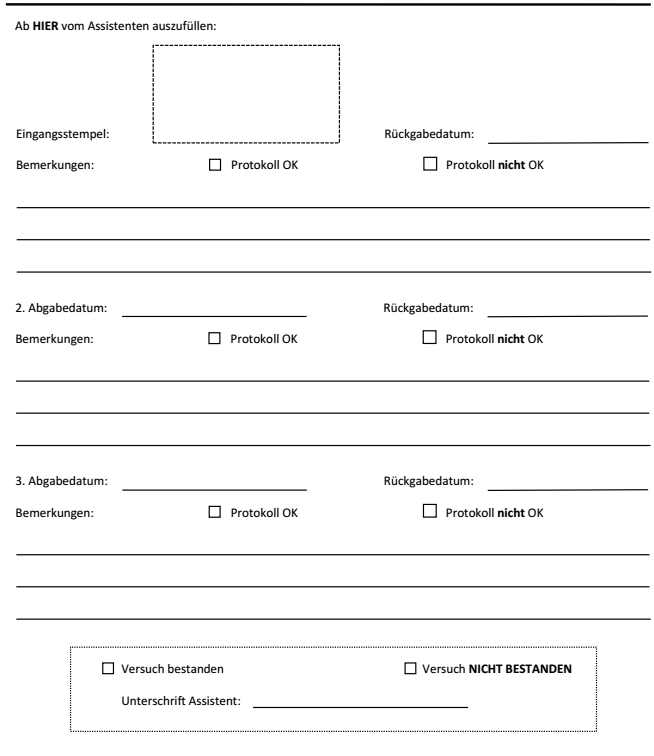
\includegraphics[width=1.1\linewidth , height=19cm]{Deckblatt_rest}}
\end{figure}

\newpage

\tableofcontents

\vspace{10pt}

\section{Aufgabenstellung}
\begin{flushleft}
Der Versuch Nr. \vnr \glqq Bestimmung der \texttt{FARADAY}-Konstante\grqq\hspace{1pt} behandelt die experimentelle Ermittlung einer physikalischen Konstanten. Für diese Aufgabe verwenden wir den \texttt{HOFFMANN}schen Wasserzersetzungsapparat.

Bei diesem Versuch gehen wir wie folgt vor:
\begin{enumerate}[label=\Roman*), itemsep=0pt]
\item Mehrere Messungen (mindestens fünf) durchführen. Hierbei sollen verschiedene Gasvolumina verwendet und Zeitdauer sowie Stromstärke variiert werden.
\item Ermitteln der \texttt{FARADAY}-Konstante aus den Messwerten und Vergleich mit Literaturwerten; anschließend die \texttt{AVOGADRO}-Konstante ermitteln.
\item Verbrauchtes Wasservolumen berechnen und erklären des Füllstandunterschiedes in den äußeren Rohrteilen.
\end{enumerate}
\end{flushleft}


\section{Messmethoden}
\begin{flushleft}
Zur Bestimmung der \texttt{FARADAY}-Konstante führen wir eine \textbf{Elektrolyse} durch. Elektrolyse bezeichnet dabei den Vorgang, bei dem mit der Hilfe von elektrischem Strom chemische Reaktionen hervorgerufen werden, sog. \textbf{Redoxreaktionen}, wodurch in unserem Fall Wassermoleküle ($H_2O$) zerteilt werden - in Sauerstoff ($O_2$) und Wasserstoff ($H_2$).
\end{flushleft}

\subsection{Physikalischer Hintergrund}
\begin{flushleft}
Die \texttt{FARADAY}-Konstante ist eine wichtige Konstante in der Physik, insbesondere den \textit{Faradayschen Gesetzen}. Die Konstante gibt die elektrische Ladung eines Mols einfach geladener Ionen an.

In diesem Versuch benutzen wir dabei diese Formel zur Berechnung des normierten Wasserstoffvolumens:

\begin{equation}\label{eq:filler}
V^{(0)} = V_{H_2} \cdot \frac{p}{p^{(0)}} \cdot \frac{T^{(0)}}{T}
\end{equation}

mit $p = p_L + \rho \cdot g \cdot h_{H_2} - 0.94 \cdot p_d$. Hierbei wurde die Druckkorrektur angewandt (Siehe auch: \hyperlink{Dkorr}{Druckkorrektur}).

Mit dem Ergebnis aus Gleichung \ref{eq:filler} können wir dann die \texttt{FARADAY}-Konstante berechnen durch:

\begin{equation}\label{eq:main}
F = \frac{I \cdot t \cdot V^{(0)}_{molar}}{2V^{(0)}}
\end{equation}

mit

\begin{itemize}[itemsep=0pt]
\item[$V_{H_2}$] = Wasserstoffvolumen [$m^3$]
\item[$p_L$] = Luftdruck [$Pa$]
\item[$\rho$] = Dichte der Elektrolytlösung [$kg / m^3$]
\item[$g$] = Erdbeschleunigung [$m / s^2$]
\item[$h_{H_2}$] = Füllstandshöhendifferenz [$m$]
\item[$p_d$] = Sättigungsdampfdruck des Wassers [$Pa$]
\item[$p^{(0)}$] = Normdruck [$Pa$]
\item[$T^{(0)}$] = Normtemperatur [$K$]
\item[$T$] = Temperatur des Elektrolyts [$K$]
\item[$I$] = Stromstärke [$A$]
\item[$t$] = Zeit [$s$]
\item[$V^{(0)}_{molar}$] = molares Volumen [$m^3 / mol$]
\item[$V^{(0)}$] = abgeschiedenes Wasserstoffvolumen bei Normbedingungen [$m^3$], hier $\cdot 2$, da zwei H-Atome je Molekül vorliegen.
\end{itemize}

Einige der benötigten Werte können wir dabei bei der Elektrolyse mit dem \texttt{HOFFMANN}schen Wasserzersetzungsapparat messen (Siehe Tabelle \ref{tab:messerg} und \ref{tab:Berechnungen}), der dazu dient, eine Elektrolyse durchzuführen. Die übrigen Parameter sind unterdessen fest (für die von uns verwendeten Materialien):
\begin{align*}
\rho &= 1.08 \cdot 10^3 kg/m^3 & g &= 9.91 m/s^2 & p^{(0)} &= 1.01325 \cdot 10^5 Pa \\ T^{(0)} &= 273.15 K & V^{(0)} &= 22.414 \cdot 10^{-3} m^3/mol
\end{align*}

Nach dem Berechnen der \texttt{FARADAY}-Konstante können wir auch die \texttt{AVOGADRO}-Konstante bestimmen, da diese Konstanten zusammenhängen durch

\begin{equation}
F = N_A \cdot e
\end{equation}
\end{flushleft}

\subsection{Genauere Betrachtung der Elektrolyse}
\begin{flushleft}
Bei der Elektrolyse von Wasser werden die Wassermoleküle in $H$ und $O$ gespalten. Dabei lässt sich ermitteln, welches Volumen an Wasser für eine Abscheidung einer bestimmten Menge Wasserstoffes (oder Sauerstoffes) notwendig ist.

\begin{figure}[h]
\centering
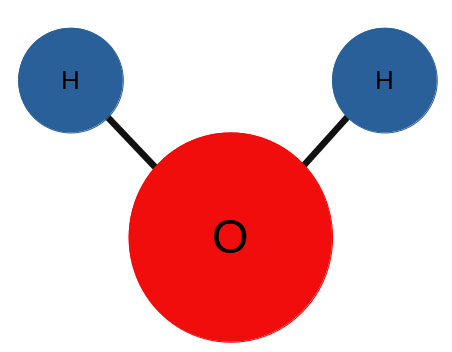
\includegraphics[scale=0.5]{Wassermolekuel}
\caption{Darstellung eines Wassermoleküls}
\label{fig:Wassmol}
\end{figure}

Ein Wassermolekül besteht aus zwei Wasserstoffatomen und einem Sauerstoffatom (Abbildung \ref{fig:Wassmol}). Die entstehenden Endprodukte sind somit Wasserstoff und Sauerstoff, wobei diese dann als $H_2$ bzw. $O_2$ vorliegen. Die Reaktion die bei der Elektrolyse abläuft beschreibt sich durch $2 H_2O \rightarrow 2 H_2 + O_2$.\footnote{Genauere Informationen \href{https://de.wikipedia.org/wiki/Wasserelektrolyse}{hier klicken}} Es fällt auf, dass immer die doppelte Menge an Wasserstoff als Sauerstoff abgeschieden wird, weshalb auch die Füllstände in den äußeren Schenkeln des Wasserzersetzungsapparates unterschiedlich sind. Bei einer idealen Elektrolyse von Wasser sollte die Differenz des Füllstandes bei Beginn des Versuches und des Füllstandes bei Ende für Wasserstoff (Kathode) genau doppelt so groß sein, wie bei Sauerstoff (Anode).

Bei einer Elektrolyse, bei der $50ml \hspace{1pt} H_2$ abgescheiden werden soll, wird also gleichzeitig $25ml \hspace{1pt} O_2$ abgestoßen, wie die reaktionsgleichung zeigt. Somit werden $75ml H_2O$ benötigt, damit $50ml H_2$ abgeschieden werden können.
\end{flushleft}

\subsection{Versuchsaufbau}
\begin{flushleft}
Die Elektrolyse führen wir mit dem \texttt{HOFFMANN}schen Wasserzersetzungsapparat durch. Dieser ist wie folgt aufgebaut:
\end{flushleft}

\begin{figure}[H]
\centering
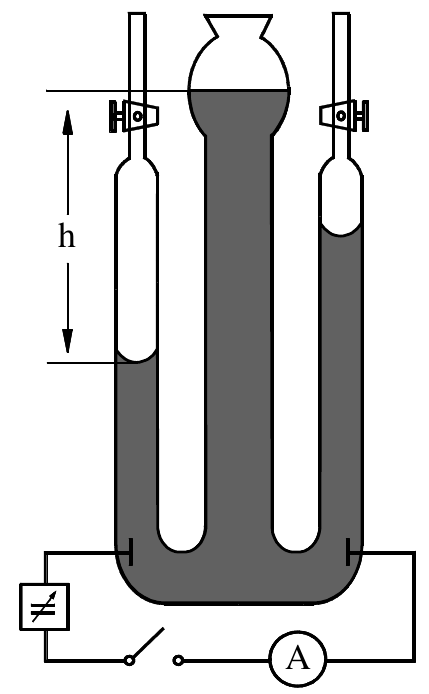
\includegraphics[scale=0.35]{VersAufbau}
\caption[Versuchsaufbau]{\texttt{HOFFMANN}sche Wasserzersetzungsapparat\footnotemark}
\label{fig:wasszersetzapa}
\end{figure}

\footnotetext{Bildquelle: \hyperlink{https://www.uni-frankfurt.de/49295051/Generic_49295051.pdf}{Anleitung zu Versuch 6 des \textit{Anfängerpraktikum \rom{2}}} des Instituts für Angewandte Physik der Goethe Universität Frankfurt am Main}

\begin{flushleft}
Für dieses Experiment benötigen wir also neben dem Wasserzersetzungsapparat zusätzlich eine Stromquelle, ein Amperemeter und einen Schalter.

Wir benötigen zudem folgende Messinstrumente zum Messen verschiedener Größen:
\begin{itemize}[itemsep=0pt]
\item Stromstärke (I): Amperemeter
\item Zeit (t): Stoppuhr
\item Luftdruck (p): Barometer
\item Temperatur (T): Thermometer
\item Volumen (V): Volumenmessgerät
\item Füllstandsdifferenz (h): Lineal
\end{itemize}
\end{flushleft}

\section{Versuchsdurchführung}
\begin{flushleft}
Für die Durchführung müssen wir zunächst den Versuchsaufbau (Abbildung \ref{fig:wasszersetzapa}) aufbauen. Wir füllen den Apparat mit destilliertem Wasser ($H_2O$), dem eine geringe Menge Schwefelsäure ($H_2SO_4$) zugesetzt wurde, um die Leitfähigkeit zu erhöhen. Bevor die Elektrolyse startet, ist es wichtig die Gashähne richtig zu schließen, da wir sonst fehlerhafte Ergebnisse erzielen.

Wir führen anschließend mehrere Messungen durch, wobei bei jeder Messung die Stromstärke und Zeitdauer variiert wird - und dadurch auch das Gasvolumen. Die Ergebnisse werden in die Tabelle \ref{tab:messerg} eingetragen.
\end{flushleft}

\section{Versuchsergebnisse}
\begin{table}[H]
\centering
\caption[Messergebnisse]{Messergebnisse}
\label{tab:messerg}
\scriptsize
\centerline{
\begin{tabular}{|c|c|c|c|c|c|c|c|c|c|c|c|}
\hline
$I (A)$ & $I_{max} (A)$ & $\Delta I (A)$ & $t (s)$ & $\Delta t (s)$ & $p_{luft} (torr)$ & $\Delta p_{luft} (torr)$ & $T_{Raum} (^{\circ}C)$ & $\Delta T (^{\circ}C)$ & $V_{H_2} (m^3)$ & $\Delta V_{H_2} (m^3)$  \\
\hline
0.5 & 1 & 0.02 & 361 & 1 & 754 & 2 & 23 & 2 & $2.56\cdot 10^{-5}$  & $2\cdot 10^{-7
}$ \\ 
\hline
0.5 & 1 & 0.02 & 490 & 1 & 754 & 2 & 23 & 2 & $3.28\cdot 10^{-5}$  & $2\cdot 10^{-7
}$ \\ 
\hline
0.2 & 1 & 0.02 & 363 & 1 & 754 & 2 & 23 & 2 & $1.5\cdot 10^{-5}$  & $2\cdot 10^{-7
}$ \\ 
\hline
0.84 & 1 & 0.02 & 104 & 1 & 754 & 2 & 23 & 2 & $1.12\cdot 10^{-5}$  & $2\cdot 10^{-7
}$ \\ 
\hline
0.2 & 1 & 0.02 & 1500 & 1 & 754 & 2 & 23 & 2 & $3.8\cdot 10^{-5}$  & $2\cdot 10^{-7
}$ \\ 
\hline
0.89 & 1 & 0.02 & 360 & 1 & 754 & 2 & 23 & 2 & $4.36\cdot 10^{-5}$  & $2\cdot 10^{-7}$ \\ 
\hline
\end{tabular}
}
\end{table}

\begin{table}[h]
\centering
\caption[Kalkulationsergebnisse]{Mess- und Kalkulationsergebnisse}
\label{tab:Berechnungen}
\scriptsize
\centerline{
\begin{tabular}{|c|c|c|c|c|c|c|c|c|c|}
\hline
$h_{H_2} (m)$ & $\Delta h_{H_2} (m)$ & $Q (C)$ & $\Delta Q (C)$ & \texttt{F} $(C / mol)$ & $\Delta$ \texttt{F} $(C / mol)$ & $V^{(0)} (m^3)$ & $\Delta V^{(0)} (m^3)$ \\
\hline
0.248 & 0.005 & 180.5 & 7.72 & 86365.562 & 7085.189 & $2.343\cdot 10^{-5}$  & $-2.15\cdot 10^{-5
}$ \\ 
\hline
0.35 & 0.005 & 245 & 10.3 & 90521.365 & 7306.152 & $3.034\cdot 10^{-5}$  & $-2.79\cdot 10^{-5
}$ \\ 
\hline
0.185 & 0.005 & 72.6 & 7.46 & 59681.868 & 11728.937 & $1.364\cdot 10^{-5}$  & $-1.244\cdot 10^{-5
}$ \\ 
\hline
0.176 & 0.005 & 87.36 & 2.92 & 96273.466 & 6139.906 & $1.017\cdot 10^{-5}$  & $-9.234\cdot 10^{-6
}$ \\ 
\hline
0.352 & 0.005 & 300 & 30.2 & 95654.617 & 18494.686 & $3.515\cdot 10^{-5}$  & $-3.236\cdot 10^{-5
}$ \\ 
\hline
0.376 & 0.005 & 320.4 & 8.09 & 88815.524 & 4308.785 & $4.043\cdot 10^{-5}$  & $-3.724\cdot 10^{-5}$ \\ 
\hline
\end{tabular}
}
\end{table}

\begin{flushleft}
Die Tabellen \ref{tab:messerg} und \ref{tab:Berechnungen} zeigen die Messergebnisse, wobei zweitere zusätzlich die berechneten Werte für die Ladung, \texttt{FARADAY}-Konstante und das normierte Wasserstoffvolumen enthält. Hierbei berechnet sich die Ladung Q durch $Q = I \cdot t$ und $\Delta Q = I \cdot \Delta t + \Delta I \cdot t$.

Weiterhin berechnet sich $\Delta V^{(0)}$ mit
\begin{align*}
\Delta V^{(0)} &= V_{H_2} \cdot \left(\frac{p}{p^{(0)}} \cdot \left(- T^{(0)} \cdot \frac{\Delta T}{T^2} \right) + \frac{\Delta p}{p^{(0)}} \frac{T^{(0)}}{T} \right) + \Delta	V_{H_2} \frac{\Delta p}{p^{(0)}} \frac{T^{(0)}}{T} \\
&= \frac{T^{(0)}}{p^{(0)} \cdot T} \cdot \left(V_{H_2} \cdot \left(- \frac{p \cdot \Delta T}{T} + \Delta p \right) + \Delta V_{H_2} \cdot p \right) \\
\end{align*}
dabei ist
\begin{align*}
p &= p_L + \rho \cdot g \cdot h_{H_2} - 0.94 p_d & \Delta p &= \Delta p_L + \rho \cdot g \cdot \Delta h_{H_2} + 0.94 \cdot \Delta p_d
\end{align*}
Wir nehmen hierbei an, es gilt $\Delta p_d = 0$, da keine Angaben zu einem absoluten Fehler dieser Größe vorliegen.

Mit diesen Ergebnissen berechnet sich dann $\Delta F$ mit
\begin{align*}
\Delta F &= \Delta Q \cdot V^{(0)}_{molar} \cdot \frac{1}{2 \cdot V^{(0)}} + 2 \cdot \Delta V^{(0)} \cdot \frac{Q \cdot V^{(0)}_{molar}}{(2 \cdot V^{(0)})^2} \\
&= \frac{V^{(0)}_{molar}}{2 \cdot V^{(0)}} \cdot \left(\Delta Q + 2 \cdot \Delta V^{(0)} \cdot \frac{Q}{2 \cdot V^{(0)}} \right) \\
\end{align*}

Außerdem können wir aus der Temperatur auf den Sättigungsdampfdruck für die Gleichung \ref{eq:filler} schließen. Da die Temperatur konstant ist, gilt für alle Messungen $p_d = 2.81 \cdot 10^{3} Pa$.
\end{flushleft}

\begin{figure}[H]
\centering
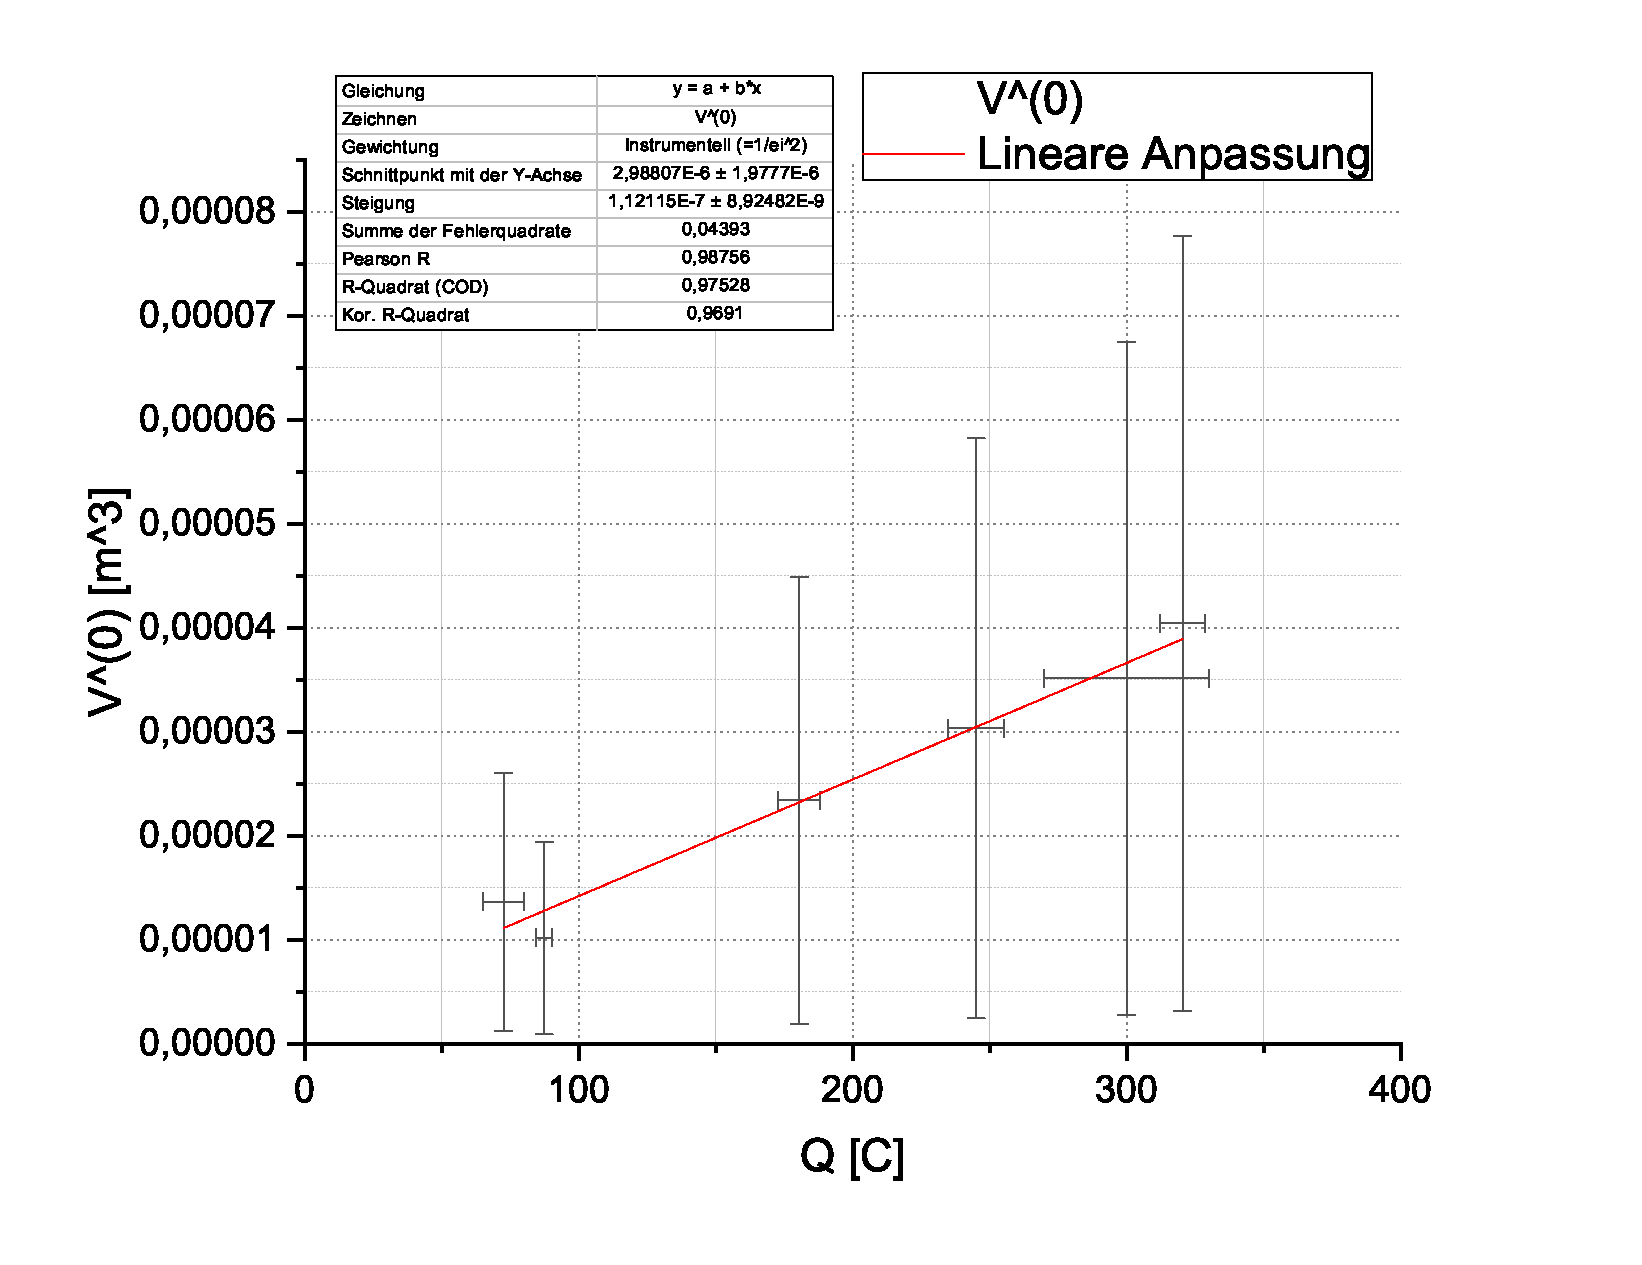
\includegraphics[scale=0.5]{Graph}
\caption[Graph: Ladung \& Wasserstoffvolumen]{Graphische Darstellung der Messdaten zu Ladung und Wasserstoffvolumen}
\label{fig:LadVol}
\end{figure}

\begin{flushleft}
Der Graph (Abbildung \ref{fig:LadVol}) zeigt das Normvolumen in Abhängigkeit der Ladung. Wir können aus der Steigung die \texttt{FARADAY}-Konstante bestimmen durch $F = \frac{1}{b} \cdot 10^{-2} \approx 89194.41 \frac{C}{mol}$ mit Steigung $b$ und Faktor $10^{-2}$ zur umrechnung von $m^3$ zu $mol$.

Den fehler können wir zudem berechnen mit $\Delta F = \pm |\frac{\Delta b}{b^2}| \approx \pm 7100.22 \frac{C}{mol}$.

Wir haben also die \texttt{FARADAY}-Konstante berechnet mit $F = (89194.41 \pm 7100.22) \frac{C}{mol}$
\end{flushleft}

\subsection{Diskussion der Messergebnisse}
\begin{flushleft}
Mit unseren ermittelten Werten je Messung für die \texttt{FARADAY}-Konstante können wir nun einen Mittelwert bilden:
\end{flushleft}

\begin{figure}[h]
\centering
\begin{subfigure}[c]{0.5\textwidth}
\subcaption{Berechnung des Mittelwertes}
\begin{align*}
\varnothing F &= \sum F_i \\
&\approx \frac{517312.37 \frac{C}{mol}}{6} \\
&\approx 86218.728 \frac{C}{mol} \\
\end{align*}
\end{subfigure}%
\begin{subfigure}[c]{0.5\textwidth}
\subcaption{Berechnung des Standardfehlers}
\begin{align*}
\sigma_{\bar{x}} &= \frac{\sigma}{\sqrt{n}} = \sqrt{\frac{\sum(F_i - \varnothing F)^2}{n-1}} \cdot \frac{1}{\sqrt{n}} \\
&= \frac{13561.83172 \frac{C}{mol}}{\sqrt{6}} \\
&\approx 5536.595 \frac{C}{mol}
\end{align*}
\end{subfigure}%
\end{figure}

\begin{flushleft}
Der Mittelwert der Messungen für die \texttt{FARADAY}-Konstante beträgt somit $(86218.728 \pm 5536.595) \frac{C}{mol}$. Der Literaturwert \cite{Farad} dieser Konstante beträgt $96485.3321233100184 \frac{C}{mol}$; die Abweichung des Berechneten Wertes beläuft sich dabei auf $10266.60412331001 \frac{C}{mol}$. Dies sind $\approx 10.64\%$. Die lineare Regression hat zudem einen Wert von $F = (89194.41 \pm 7100.22) \frac{C}{mol}$ ergeben. Dieser Wert ist noch näher an dem Literaturwert.


Mit dem ermittelten Mittelwert können wir nun die \texttt{AVOGADRO}-Konstante bestimmen durch

\begin{equation*}
F = N_A \cdot e \Rightarrow N_A = \frac{F}{e}
\end{equation*}

Hierbei beschreibt $e$ die Elementarladung ($\approx 1.602176 \cdot 10^{-19} C$).
\end{flushleft}

\begin{figure}[h]
\centering
\begin{subfigure}[c]{0.5\textwidth}
\subcaption{Berechnung des Mittelwertes}
\begin{align*}
N_A &= \frac{F}{e} \\
&= \frac{86218.728 \frac{C}{mol}}{1.602176 \cdot 10^{-19} C} \\
&\approx 5.381 \cdot 10^{23} mol^{-1} \\
\end{align*}
\end{subfigure}%
\begin{subfigure}[c]{0.5\textwidth}
\subcaption{Berechnung des absoluten Fehlers}
\begin{align*}
\Delta N_A &= \frac{\Delta F}{e} \\
&= \frac{5536.595 \frac{C}{mol}}{1.602176 \cdot 10^{-19} C} \\
&\approx 0.3456 \cdot 10^{23} mol^{-1} \\
\end{align*}
\end{subfigure}%
\end{figure}

\begin{flushleft}
Unsere Messungen ergeben somit einen Wert der \texttt{AVOGADRO}-Konstante von $(5.381 \pm 0.3456) \cdot 10^{23} mol^{-1}$. Der Literaturwert \cite{Avocado} für diese Konstante beträgt $6.02214076 \cdot 10^{23} mol^{-1}$. Unser Wert weicht um $\approx 0.6408 \cdot 10^{23} mol^{-1}$ bzw. $\approx 10.64\%$ vom Literaturwert ab.
\end{flushleft}

\subsection{Fehlerbetrachtung}
\begin{flushleft}
Der Vergleich der berechneten Werte für \texttt{FARADAY}- und \texttt{AVOGADRO}-Konstante mit den jeweiligen Literaturwerten hat gezeigt, dass unsere Berechnungen durchaus stark abweichen (10\%, bzw. 51\%). Diese Abweichungen können durch verschiedene Fehlerquellen verursacht werden:

\begin{itemize}
\item Um die Leitfähigkeit des Wassers zu steigern, haben wir dieses mit geringen Mengen Schwefelsäure ($H_2SO_4$) versetzt. Die hat jedoch den Nebeneffekt, dass bei der Elektrolyse Peroxydschwefelsäure ($H_2S_2O_8$) gebildet werden kann. Nebenbei können die Sauerstoffatome auch Ozon ($O_3$) bilden und sind dazu auch sehr löslich in Wasser. Aus diesem Grund haben wir das Volumen des Wasserstoffes und dessen Höhendifferenz gemessen, anstatt des Sauerstoffes.
\item Bei der Spaltung des Wassers steigen die gespaltenen Moleküle als Bläschen zu sehen nach oben. Dabei können vereinzelt Bläschen hängen bleiben. Im Fall, dass diese an der Anode oder Kathode hängen bleiben, kann dies zur weiteren (stärkeren) Erwärmung des Apparats führen und dabei auch zu einer höheren Abscheidung von Gasen bei höheren Stromstärken.
\item \hypertarget{Dkorr}{Generell} kann es bei Messungen auch zu Messfehlern kommen oder die Werte nicht korrekt abgelesen werden, wobei diese in den genutzten Formeln bestmöglich berücksichtigt wurde, u.a. mit der Druckkorrektur:
\begin{equation*}
p_L + \rho \cdot g \cdot h - 0.94 \cdot p_d
\end{equation*}
\end{itemize}
\end{flushleft}

\section{Fazit}
\begin{flushleft}
Der Versuch \vnr \hspace{1pt} \glqq Bestimmung der \texttt{FARADAY}-Konstante\grqq \hspace{1pt} ist ein interessanter Versuch. Es wurde u.a. der Ablauf einer Elektrolyse betrachtet, sowie der Zusammenhang einiger physikalischen Konstanten. Ersteres hat dabei einen sehr aktuellen Bezug, da im Moment ein hohes Interesse an regenerativen und umweltschonenden Methoden zur Energieumwandlung und -speicherung besteht (z.B. der \textit{Brennstoffzelle}).
\end{flushleft}

\begingroup
\raggedright
\sloppy
\printbibliography[heading=bibintoc,title={7 \hspace{6pt} Literatur}]
\endgroup
\end{document}
